\documentclass[fontsize=12pt,paper=a4,twoside]{scrartcl}

\newcommand{\grad}{\ensuremath{^{\circ}} }
\renewcommand{\strut}{\vrule width 0pt height5mm depth2mm}

\usepackage[utf8]{inputenc}
\usepackage[final]{pdfpages}
% obere Seitenränder gestalten können
\usepackage{fancyhdr}
\usepackage{moreverb}
% Graphiken als jpg, png etc. einbinden können
\usepackage{graphicx}
%\usepackage{stmaryrd}
% Floats Objekte mit [H] festsetzen
\usepackage{float}
% setzt URLs schön mit \url{http://bla.laber.com/~mypage}
\usepackage{url}
% Externe PDF's einbinden können
\usepackage{pdflscape}
% Verweise innerhalb des Dokuments schick mit " ... auf Seite ... "
% automatisch versehen. Dazu \vref{labelname} benutzen
\usepackage[ngerman]{varioref}
\usepackage[ngerman]{babel}
\usepackage{ngerman}
% Bibliographie
\usepackage{bibgerm}
% Tabellen
\usepackage{tabularx}
\usepackage{supertabular}
\usepackage[colorlinks=true, pdfstartview=FitV, linkcolor=blue,
            citecolor=blue, urlcolor=blue, hyperfigures=true,
            pdftex=true]{hyperref}
\usepackage{bookmark}
\usepackage{enumitem}

\newboolean{langversion} %Deklaration
\setboolean{langversion}{true} %Zuweisung ist 'false' für Blockkurs
\newcommand{\highlight}[1]{\textcolor{blue}{\textbf{#1}}}
\newcommand{\nurlangversion}[0]{%
\ifthenelse{\boolean{langversion}}{\highlight{Muss in SWP-2 ausgefüllt werden}}{\highlight{Entfällt in SWP-1}}}

\newcommand{\swp}[0]{\ifthenelse{\boolean{langversion}}%
{Software--Projekt 2}{Software--Projekt 1}}
\newcommand{\jahr}[0]{2014}
\newcommand{\semester}[0]{\ifthenelse{\boolean{langversion}}{WiSe}{SoSe}}

% Damit Latex nicht zu lange Zeilen produziert:
\sloppy
%Uneinheitlicher unterer Seitenrand:
%\raggedbottom

% Kein Erstzeileneinzug beim Absatzanfang
% Sieht aber nur gut aus, wenn man zwischen Absätzen viel Platz einbaut
\setlength{\parindent}{0ex}

% Abstand zwischen zwei Absätzen
\setlength{\parskip}{1ex}

% Seitenränder für Korrekturen verändern
\addtolength{\evensidemargin}{-1cm}
\addtolength{\oddsidemargin}{1cm}

\bibliographystyle{gerapali}

% Lustige Header auf den Seiten
  \pagestyle{fancy}
  \setlength{\headheight}{70.55003pt}
  \fancyhead{}
  \fancyhead[LO,RE]{\swp\\ \semester{}
  \\Anforderungsspezifikation}
  \fancyhead[LE,RO]{Seite \thepage\\\slshape \leftmark\\\slshape \rightmark}

%Abstände zwischen Tabellenzeilen etwas erhöhen
\renewcommand{\arraystretch}{1.2}

%
% Und jetzt geht das Dokument los....
%

\begin{document}

% Lustige Header nur auf dieser Seite
  \thispagestyle{fancy}
  \fancyhead[LO,RE]{ }
  \fancyhead[LE,RO]{Universität Bremen\\FB 3 -- Informatik\\
  Prof. Dr. Rainer Koschke \\TutorIn: Karsten Hölscher}
  \fancyfoot[C]{}

% Start Titelseite
  \vspace{3cm}

  \begin{minipage}[H]{\textwidth}
  \begin{center}
  \bf
  \Large
  \swp{} \jahr\\
  \smallskip
  \small
  VAK 03-BA-901.02\\
  \vspace{3cm}
  \end{center}
  \end{minipage}
  \begin{minipage}[H]{\textwidth}
  \begin{center}
  \vspace{1cm}
  \bf
  {\Large Anforderungsspezifikation}\\
  \vspace{3ex}
    \begin{figure}[H]
    \centering
    \includegraphics[width=0.25\textwidth]{../woym.png}
    \end{figure}
  \vfill
  \end{center}
  \end{minipage}
  \vfill
  \begin{minipage}[H]{\textwidth}
  \begin{center}
  \sf
  \begin{tabular}{l}
  Tim Hansen \\
  Joshua Hoffmann\\
  Hassan Klait \\
  Adrian Lück \\
  Jurij Schmidt\\
  Falko Schröder
  \end{tabular}
  \\ ~
  \vspace{2cm}
  \\
  \it Version 1.3\\ ~
  \end{center}
  \end{minipage}

% Ende Titelseite

% Start Leerseite

\newpage

  \thispagestyle{fancy}
  \fancyhead{}
  \fancyhead[LO,RE]{\swp{}\\ \semester{} \jahr{}
  \\Anforderungsspezifikation}
  \fancyhead[LE,RO]{Seite \thepage\\\slshape \leftmark\\~}
  \fancyfoot{}
  \renewcommand{\headrulewidth}{0.4pt}
  \tableofcontents

\newpage

  \fancyhead[LE,RO]{Seite \thepage\\\slshape \leftmark\\\slshape \rightmark}


%%%%%%%%%%%%%%%%%%%%%%%%%%%%%%%%%%%%%%%%%%%%%%%%%%%%%%%%%%%%%%%%%%%%%%%%
\section*{Version und Änderungsgeschichte}

\begin{tabularx}{\textwidth}{ccX}
Version & Datum & Änderungen \\
\hline
1.0 & 29.10.2014 & Anforderungsspezifikation als \LaTeX Vorlage kopiert. \\
1.1 & 31.10.2014 & Julia Meyer als Persona für Anwendungsfälle hinzugefügt\\ 
1.2 & 01.11.2014 & Auflistung der Verwaltung von Klassen und Personal betreffenden
				   Anwendungsfälle. Detaillierte Beschreibung des Anwendungsfalls \ref{subsubsec:KlasseHinzufuegen} (noch ohne Aktionen).\\
1.3 & 02.11.2014 & Kurzbeschreibung der Personal betreffenden Anwendungsfälle. Detaillierte
				   Beschreibung der Anwendungsfälle \ref{subsubsec:KlasseBearbeiten} und \ref{subsubsec:KlasseLoeschen} (noch ohne Aktionen).\\
\end{tabularx}


%%%%%%%%%%%%%%%%%%%%%%%%%%%%%%%%%%%%%%%%%%%%%%%%%%%%%%%%%%%%%%%%%%%%%%%%
\section{Einleitung}

\subsection{Vorbemerkung}
Im folgenden wird für Personen des Personals die weibliche Form benutzt, da Frauen an der Grundschule die deutliche Mehrheit bilden. In jedem Fall sind aber auch männliche Lehrer angesprochen.

\subsection{Zweck}
\nurlangversion

  {\em Was ist der Zweck dieser Anforderungsspezifikation? Wer sind
  die LeserInnen?}

\subsection{Rahmen}
\nurlangversion

  {\em Dieser Abschnitt soll einen groben Überblick über die zu
  erstellende Software geben: Welche Produkte sind zu erstellen (mit
  Namen)? Was tut die Software? Auch: Was tut sie nicht? Wozu soll die
  Software verwendet werden?  (Ziele etc.)}

\subsection{Definitionen, Akronyme und Abkürzungen}
\nurlangversion

  {\em Hier geht es vor allem um Begriffe aus der Anwendungsdomäne,
  d.h.\ aus der Welt des Kunden. Aber auch Begriffe, die dem Kunden
  evtl.\ fremd oder unklar sind, sollten erläutert werden.}


\subsection{Referenzen}
  {\em Neben sonstigen Quellen, die Ihr verwendet habt, können dies
  z.B.\ das Skript, dieses Beispieldokument, der zugrunde
  liegende IEEE-Standard und anderes sein}
  

\subsection{Übersicht über das Dokument}
\nurlangversion

  {\em Was enthält die Anforderungsspezifikation? Wie ist das Dokument
  organisiert?}


\section{Allgemeine Beschreibung}
\label{ch:AllgemeineBeschreibung}

\subsection{Ergebnisse der Ist-Analyse}
\nurlangversion

  {\em Hier sollten die Ergebnisse Eurer Ist-Analyse kurz
  zusammengefasst werden. Diese Beschreibung ist hilfreich, um die
  Motivation für die Anforderungen zu verstehen und um sie später
  nachzuvollziehen (z.B.\ dann wenn Anforderungen überarbeitet werden
  sollen, weil sich ihre Rahmenbedingungen geändert haben).
  
  Mögliche Inhalte: 
  \begin{itemize}
    \item Interview/Beobachtung des Kunden oder der Benutzer
    \item Analyse des bisherigen Systems und dessen Probleme 
    \item Analyse ähnlicher Systeme
    \item Auswertung der Benutzerbefragung
    \item Wie sollen die identifizierten Probleme vom neuen System adressiert werden?
  \end{itemize}
  
  N.B.: Dieser Abschnitt ist im IEEE-Standard nicht vorgesehen, aber dennoch
  sinnvoll.}

\subsubsection{Erstes Kundengespräch vom TT.MM.JJJJ}
\nurlangversion

\subsubsection{Interview mit einem Mitarbeiter der ...}
\nurlangversion

{\em Falls durchgeführt}

\subsection{Produktperspektive}
\nurlangversion
  
\subsubsection{Systemschnittstellen}
\nurlangversion

  {\em Schnittstellen zu anderen Systemen, z.B.\ Datenimport/-export,
  Konfigurationsdateien, anzubindende externe Dienste und deren Schnittstelle,
  Anbieten der eigenen Funktionalität als API o.ä.}
  

\subsubsection{Benutzerschnittstelle}
\nurlangversion

  {\em GUI-Design-Richtlinien und Interaktionsmechanismen (nicht
  Screenshots aller Dialoge --- die werden in Kapitel 3 gezeigt --- aber
  evtl.\ ein Screenshot, der einen groben Überblick und Eindruck des
  GUI-Designs gibt).}


\subsubsection{Hardwareschnittstellen}
\nurlangversion

  {\em Schnittstellen zu vorgegebenen Hardwarekomponenten (Name,
  Version).}
 

\subsubsection{Softwareschnittstellen}
\nurlangversion

{\em Softwarebibliotheken und --rahmenwerke (Frameworks), die benutzt
  werden sollen, mit Versionsnummer, Hersteller, Quelle etc. Dazu
  gehört auf jeden Fall Java.}

  \begin{tabular}{|l|l|l|l|}\hline
    \textbf{Name} & \textbf{Version} & \textbf{Hersteller} & \textbf{Quelle} \\\hline
    Java Runtime & 6 Update 37 & Oracle & \url{http://java.com} \\\hline
    Hibernate & 4.3.0.Beta1 Release& JBoss Community &  
   \url{http://www.hibernate.org/}\\\hline
    \ldots & & & \\\hline
  \end{tabular}

\subsubsection{Kommunikationsschnittstellen}
\nurlangversion

{\em Anforderungen an und Bandbreite von Kommunikationsnetzwerken, öffentliche
  oder auch private IP-Adressen?}

\subsubsection{Speicherbeschränkung}
\nurlangversion

  {\em min./max.\ verfügbarer Hauptspeicher und Festplattenplatz, knappe Begründung wie Ihr zu
der hier angegebenen Einschätzung gekommen seid}

\subsubsection{Operationen (Betriebsmodi)}
\nurlangversion

  {\em Welche Betriebsmodi gibt es? Warum? Welche Benutzerklasse darf
  was in welchem Betriebsmodus (Rechte)? Was ist der Zusammenhang
  zwischen Betriebsmodus und Sicherung/Wiederherstellung von Daten?}

\subsubsection{Möglichkeiten der lokalen Anpassung}
\nurlangversion

  {\em Was kann bei Auslieferung des Systems alles konfiguriert
  werden? Z.B. Pfade, Datenbankname, Server-IP usw. Hier ist nicht
  Internationalisierung gemeint!}


\subsection{Anwendungsfälle}
  {\em Auflistung und kurze Beschreibung aller relevanten
  Anwendungsfälle. Dies soll einen Überblick über alle Anwendungsfälle
  geben, die in 3.2 detailliert beschrieben werden.}
  
\subsubsection{Verwaltung der Klassen betreffende Anwendungsfälle}

%\paragraph{Mehrere Klassen hinzufügen} Die Anwenderin kann in der Verwaltungs-Ansicht einen Dialog öffnen, um mehrere Klassen hinzuzufügen, sofern noch keine Klassen existieren. Dazu muss lediglich die Anzahl der zu generierenden Klassen für die jeweiligen Jahrgänge angegeben werden. Das System generiert daraus die Klassenbezeichnungen, die aus Jahrgang und Klein- bzw. Großbuchstabe bestehen.

\paragraph{Klasse hinzufügen} Die Anwenderin kann in der Verwaltungs-Ansicht einzelne Klassen hinzufügen. Dazu wählt sie im entsprechenden Dialog den Jahrgang und den Bezeichner in Form eines Klein-/Großbuchstaben aus. Es können auch die Unterrichtsbedarfe der konkreten Klassen angepasst und allgemeine Bemerkungen angegeben werden.

\paragraph{Klasse bearbeiten} Die Anwenderin kann eine bestehende Klasse bearbeiten. Alle Parameter lassen sich ändern.

\paragraph{Klasse(n) löschen} Die Anwenderin kann eine oder mehrere Klassen löschen.

\subsubsection{Verwaltung des Personals betreffende Anwendungsfälle}

\paragraph{Lehrerin hinzufügen}
Die Anwenderin kann in der Verwaltungsansicht Lehrerinnen hinzufügen. Dazu müssen mindestens Vorname, Nachname, Kürzel und Anzahl der Wochenstunden (in Unterrichtsstunden) angegeben werden. Zusätzlich können Zeitwünsche, Bemerkungen und anrechenbare Ersatzleistungen erfasst werden.

\paragraph{Lehrerin bearbeiten}
Die Anwenderin kann alle Parameter einer bestehenden Lehrerin ändern.

\paragraph{Lehrerin löschen}
Die Anwenderin kann eine vorhandene Lehrerin löschen.

\paragraph{Pädagogische Mitarbeiterin hinzufügen}
Die Anwenderin kann in der Verwaltungsansicht eine pädagogische Mitarbeiterin hinzufügen. Dazu müssen wie bei der Lehrerin mindestens Vorname, Nachname, Kürzel und Anzahl der Wochenstunden in Zeitstunden angegeben werden. Auch hier können zusätzlich Zeitwünsche, Bemerkungen und anrechenbare Ersatzleistungen erfasst werden.

\paragraph{Pädagogische Mitarbeiterin bearbeiten}
Die Anwenderin kann alle Parameter einer bestehenden pädagogischen Mitarbeiterin ändern.

\paragraph{Pädagogische Mitarbeiterin löschen}
Die Anwenderin kann eine bestehende pädagogische Mitarbeiterin löschen.

\subsubsection{Verwaltung der Aktivitätstypen betreffende Anwendungsfälle}

\subsubsection{Die Stundenplan-Erstellung betreffende Anwendungsfälle}

\subsubsection{Sonstige Anwendungsfälle}

\subsection{Charakteristika der Benutzer}

\begin{tabular}{p{3cm}l}
\textbf{Name:} & Julia Meyer \\
\textbf{Alter:} & 36 Jahre\\
\textbf{Tätigkeit:} &  Grundschullehrerin\\
\end{tabular} \\

Frau Meyer ist Grundschullehrerin und unterrichtet hauptsächlich Deutsch, Englisch, Mathe und Musik. Schon früh hat sie sich für diesen Beruf entschieden und auch wenn die Kinder gelegentlich anstrengend sind, hat sie dennoch viel Spaß an ihrer Arbeit.\\
Sie möchte als Hauptverantwortliche die Planung mit der neuen Stundenplansoftware übernehmen, die einige Studierende im Rahmen der Veranstaltung ,,Software-Projekt 2`` für ihre Schule entwickeln sollen, da sie gerne sehen möchte, wie dies von den Studierenden umgesetzt wurde und sie sich erhofft diesen hilfreiches Feedback geben zu können. Nicht zuletzt erhofft sie sich aber auch, dass die neue Software den Planungsprozess deutlich beschleunigt und den Personalbedarf für diesen verringert, so dass sie und ihre Kolleginnen sich stärker auf die Betreuung der Kinder fokussieren können.  \\
Sehr wichtig ist ihr, dass die Software übersichtlich und leicht verständlich ist, denn selbst wenn man wie sie im Umgang mit PCs einigermaßen fit ist, gibt es doch nichts schlimmeres als eine chaotische Software. Da sie in Zukunft hauptverantwortlich für die Planung sein wird, hofft sie auch darauf, dass sie von der Software ausreichend unterstützt wird. Sie wünscht sich z.B. gewarnt zu werden, wenn bei der Planung das Wochenstundenkontingent einer Mitarbeiterin überschritten wird, wenn sie die Zeitwünsche einer Kollegin nicht beachtet hat oder wenn sie versucht eine Kollegin zur selben Zeit für zwei verschiedene Aktivitäten zuzuordnen. \\

\subsection{Einschränkungen}
\label{sec:Einschraenkungen}
{\em Dieser Abschnitt gibt einen groben Überblick über alles, was den
  Entwurf einschränken könnte. Details folgen dann in
  Abschnitt~\ref{ch:DetaillierteBeschreibung} (\glqq Detaillierte
  Beschreibung\grqq). Allgemeine Sicherheitsanforderungen könnten also
  hier kurz beschrieben werden, Details dann im
  Abschnitt~\ref{sec:softwaresystemattribute} zu Systemattributen.

  Beispiele für mögliche Einschränkungen könnten sein (die Liste ist
  nicht vollständig und nicht alle dieser Punkte sind in jedem
  möglichen Projekt relevant):

  \begin{itemize}
   \item feste Vorgaben (z.B. Policies)
   \item gesetzliche Rahmenbedingungen (z.B. Datenschutzaspekte)
   \item Hardwarebeschränkungen
   \item festgelegte Schnittstellen zu anderen Anwendungen
   \item parallele Operationen (z.B. Multithreading)
   \item zu unterstützende Prüffunktionen (auch: Audit-Funktionen;
     z.B. \glqq alle Buchungen im System müssen protokolliert und von
     einem Wirtschaftsprüfer nachvollziehbar sein\grqq)
   \item Steuerungsfunktionen (z.B. \glqq Das System kann von einem
     Techniker von Ferne gewartet werden\grqq)
   \item Anforderungen an die zu verwendende Programmiersprache
   \item Verlässlichkeit; die Verfügbarkeit eines technischen Systems 
       ist die Wahrscheinlichkeit oder das Maß, dass das System 
       bestimmte Anforderungen innerhalb eines vereinbarten
       Zeitrahmens erfüllt. Eine Beispielanforderung könnte sein, dass
       das System an jedem Tag der Woche 24 h lang in Betrieb sein 
       muss und im Jahr höchstens 2 Tage nicht verfügbar sein darf.
   \item Zuverlässigkeit; Software-Zuverlässigkeit wird definiert 
      als die Wahrscheinlichkeit einer fehlerfreien Software-Anwendung 
      über eine spezifizierte Zeitdauer und unter spezifizierten
      Umgebungsbedingungen. Hier könnte zum Beispiel eine zu
      erreichende Testabdeckung in Bezug auf ein Abdeckungsmaß
      gefordert werden: \glqq 90\,\% Anweisungsabdeckung bei den
      Komponententests\grqq.
   \item Kritikalität (Gefährlichkeit eines Versagens) der Anwendung
   \item Sicherheit
  \end{itemize}

}

\subsubsection{Rahmenbedingungen}
\nurlangversion

\subsubsection{Gesetzliche Rahmenbedingungen}
\nurlangversion
 
\subsubsection{Sicherheitskritische Aspekte}
\nurlangversion

\subsection{Annahmen und Abhängigkeiten}
\nurlangversion

  {\em Faktoren, deren Änderung zwangsläufig zu Änderungen an der
  Anforderungsspezifikation führen würde.}



\subsection{Ausblick}
\nurlangversion

  {\em Beschreibt hier knapp, welche Änderungen und Erweiterungen
  zukünftig (d.h.\ nach Auslieferung des Systems) zu erwarten sind.
  Diese Information ist wichtig für den Entwurf, um mögliche
  Änderungen frühzeitig im ersten Entwurf berücksichtigen zu können.
  Der Entwurf kann dann so gestaltet werden, dass die zukünftigen
  Anforderungen leicht realisierbar sind. Die zukünftigen
  Anforderungen sollten realistisch sein, ansonsten könnte ein unnötig
  allgemeiner und damit zu komplizierter Entwurf die Folge sein.  Auch
  dieser Abschnitt ist im IEEE-Standard nicht vorgesehen -- zumindest
  nicht explizit in Form eines eigenständigen Abschnitts. Dennoch
  handelt es sich um wertvolle Information, von der der Entwurf
  profitieren kann.}
  

\section{Detaillierte Beschreibung}
\label{ch:DetaillierteBeschreibung}
{\em Die externen Schnittstellen werden grob in Abschnitt 2
  beschrieben.  Wenn die grobe Beschreibung dort nicht genügt, kann
  sie hier detaillierter ausgeführt werden (wie vom IEEE-Standard
  vorgesehen).}

\subsection{Datenmodell}
  {\em Das Datenmodell im Kontext des Pflichtenhefts ist {\glqq}die
  Darstellung von Informationen und deren Beziehungen in einem
  fachlogischen Konzept{\grqq}. Es soll hier gezeigt werden, welche
  Einheiten für das existierende System relevant sind und welche
  Beziehungen zwischen diesen Einheiten gelten. Es handelt sich
  hierbei noch nicht um ein Datenbankschema oder eine Spezifikation
  von Klassen für die Implementierung (Entwurf), sondern um die
  Modellierung der realen Welt. Das Datenmodell ist leitend für den
  Entwurf (weil alles darin beschrieben sich auch in der Software 
  wiederfinden wird), aber nimmt den Entwurf nicht schon vorweg.
  
  Das Datenmodell soll als UML-Klassendiagramm angegeben werden.
  Wichtig ist hierbei die korrekte Verwendung der UML: Klassen,
  Attribute, Generalisierung, Assoziation, Aggregation, Komposition,
  Multiplizitäten. Außerdem sollte das Diagramm sinnvoll und gut
  lesbar sein. Dazu gehört weiterhin eine kurze Beschreibung des
  Modells mit ergänzenden Informationen, insbesondere wenn die
  Relationen durch ihren Namen nicht selbsterklärend sind. Gebt
  unbedingt ein Mengengerüst für die Daten an: Wie viele Instanzen der
  wichtigsten Klassen werden erwartet? Erwartet Ihr Änderungen im
  Datenvolumen in der Zukunft?}


\subsection{Anwendungsfälle}

\subsubsection{Anmerkungen zur Notation}
Bei Varianten und Fehler- und Ausnahmefällen dient die numerische Aufzählung auf erster Ebene lediglich der Unterscheidung der Varianten bzw. Fehler- und Ausnahmefällen. Eine numerische Aufzählung auf zweiter oder höherer Ebene beschreibt einen chronologischen Ablauf und eine alphabetische Aufzählung auf zweiter oder höherer Ebene stellt Subvarianten dar.
  
\subsubsection{Abbildungen}

\begin{figure}[H]
\caption{Verwaltungsansicht}
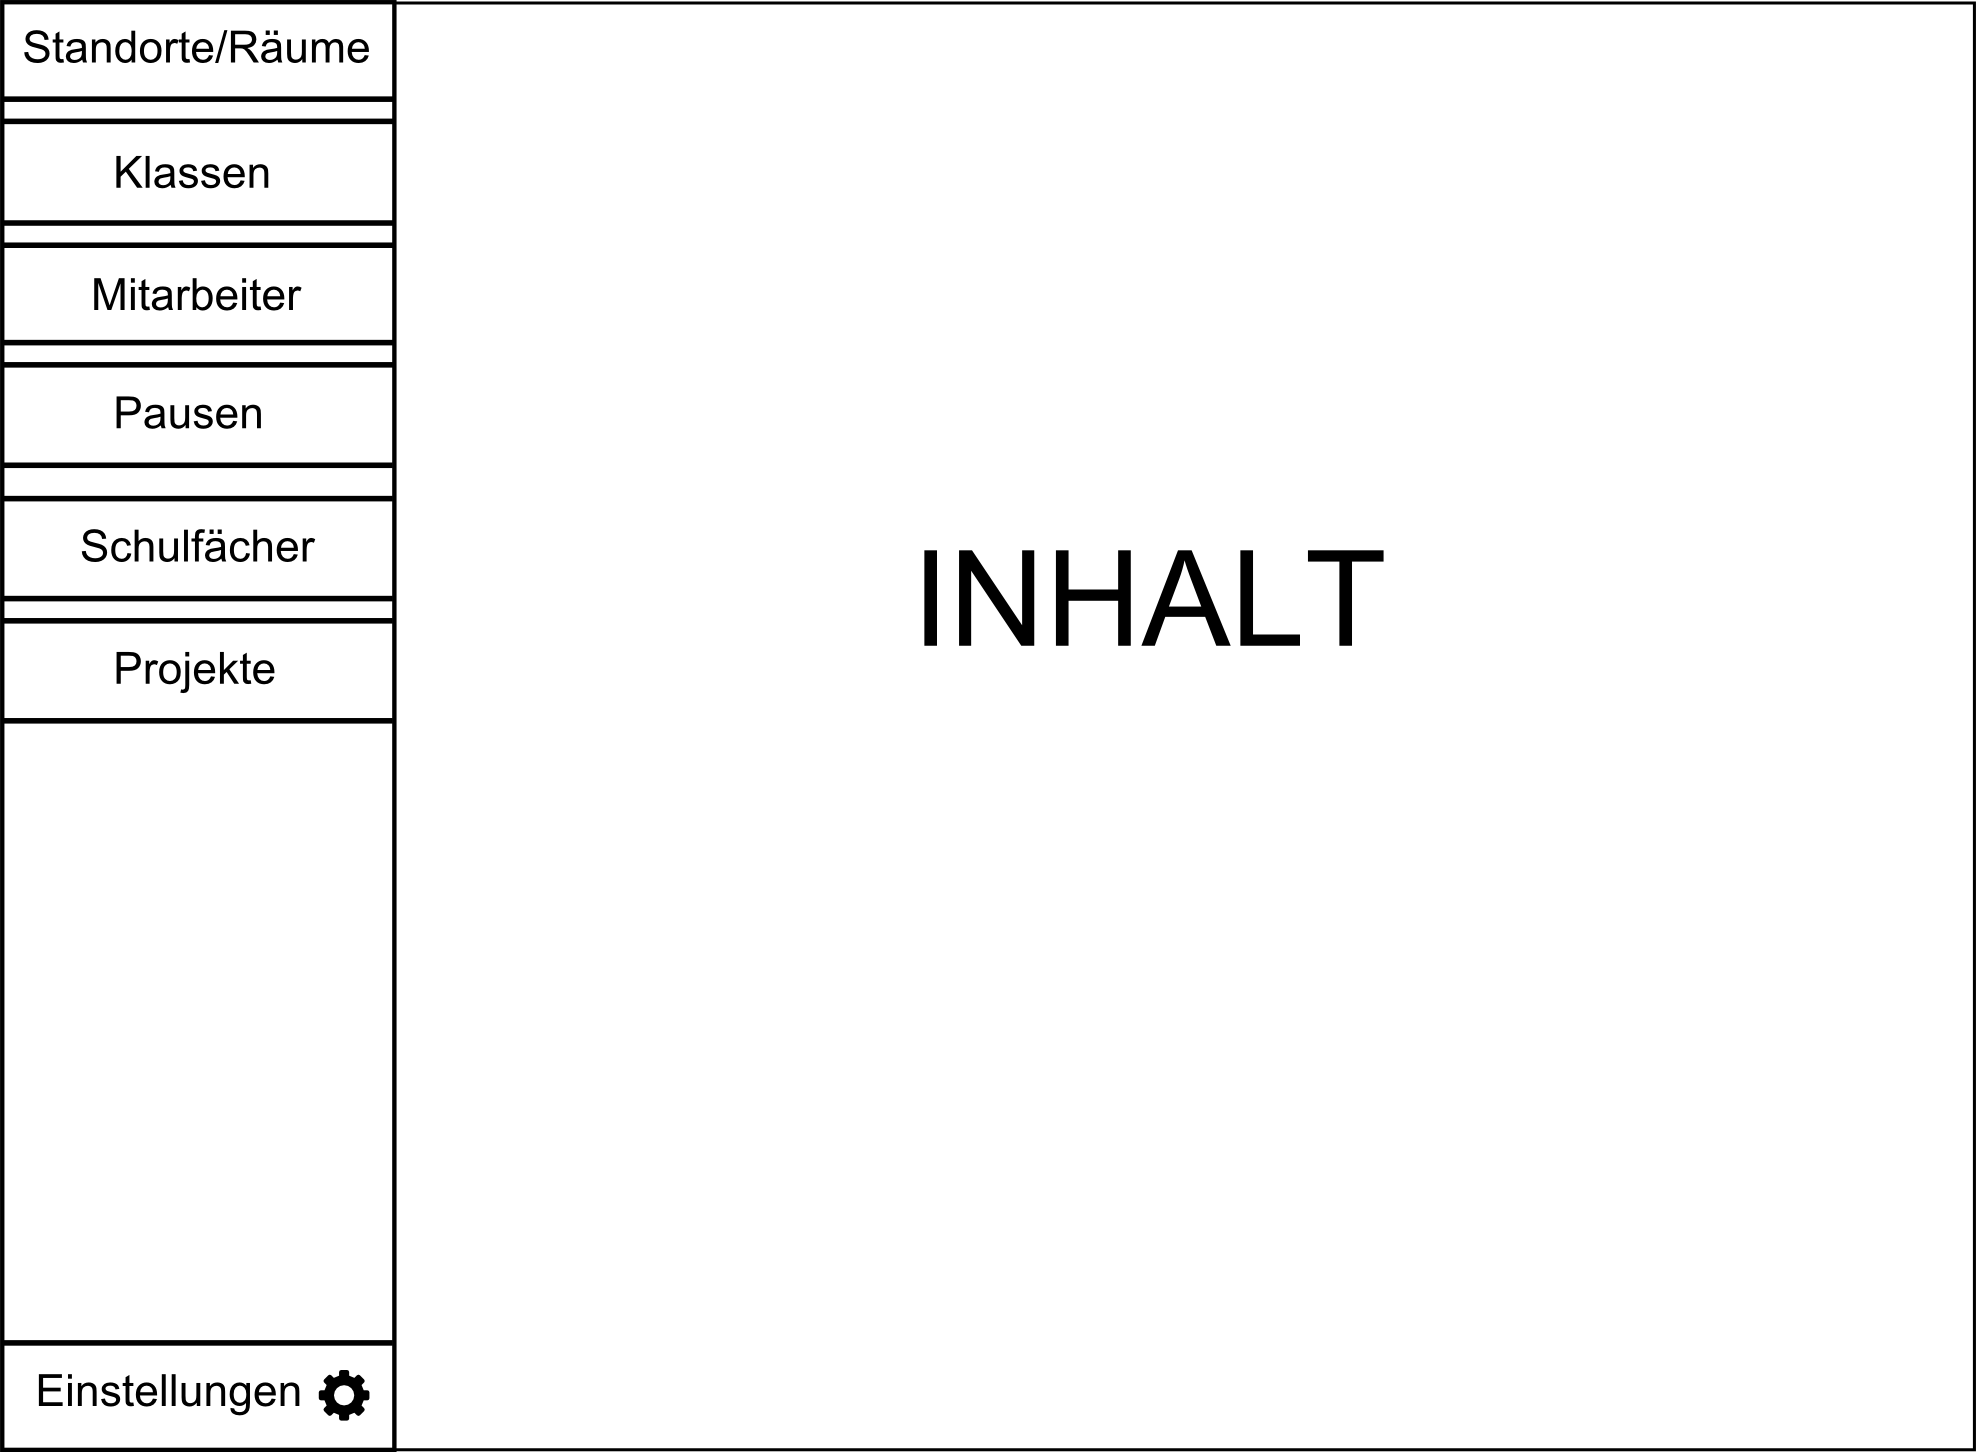
\includegraphics[width=0.75\textwidth]{mainpage_idea.png}
\end{figure}
\vspace{5pt}


\label{subsubsec:KlasseHinzufuegen}
\subsubsection{Klasse hinzufügen}

\textbf{Akteurin}
\begin{itemize}
\item Julia Meyer
\end{itemize}
\vspace{5pt}


\textbf{Vorbedingungen}
\begin{enumerate}
\item Die Software wurde von Frau Meyer gestartet und sie befindet sich in der Verwaltungs-Ansicht (s. Abb. 1).
\item Es wurden bereits Schulfächer hinzugefügt.
\item Es sind Unterrichtsbedarfe für die jeweiligen Jahrgänge vorhanden.
\item Es wurden bereits Räume hinzugefügt.
\end{enumerate}
\vspace{5pt}


\textbf{Nichterfüllung von Vorbedingungen}
\begin{itemize}
\item Nichterfüllung von Vorbedingung 2 und 3: Es können keine Unterrichtsbedarfe angegeben werden.
\item Nichterfüllung von Vorbedingung 3: Es können keine dem Jahrgang entsprechenden Unterrichtsbedarfe geladen werden. Eine individuelle Angabe von Unterrichtsbedarfen ist aber möglich, wenn Vorbedingung 2 erfüllt ist.
\item Nichterfüllung von Vorbedingung 4: Es kann kein Klassenraum angegeben werden.
\end{itemize}
\vspace{5pt}

\textbf{Regulärer Ablauf}
\begin{enumerate}
\item Frau Meyer klickt im Navigationsmenü auf der linken Seite auf den Menüpunkt ,,Klassen``.
\item Daraufhin werden im rechten Feld (s. Abb. 1) eine Liste der vorhandenen Klassen, sowie Buttons für das Hinzufügen, Bearbeiten und Löschen der Klassen angezeigt.
\item Frau Meyer klickt auf den ,,Hinzufügen``-Button.
\item Es öffnet sich ein modaler ,,Klasse hinzufügen``-Dialog.
\item Frau Meyer wählt in einer Liste den vierten Jahrgang aus. 
\item In einer zweiten Liste werden alle noch verfügbaren Bezeichner für diesen Jahrgang angezeigt.
\item Frau Meyer wählt als Bezeichner ,,A``.
\item Das System lädt die  Unterrichtsbedarfe für den vierten Jahrgang ($\rightarrow$ \texttt{Lade Unterrichtsbedarfe}) und stellt diese im Dialog dar.
\item Frau Meyer möchten den optional anzugebenden Klassenraum auswählen. Sie wählt aus einem Drop-Down-Menü Raum ,,101 (Standort A)`` aus.
\item Frau Meyer möchte die Unterrichtsbedarfe nicht anpassen.
\item Frau Meyer klickt auf den ,,OK``-Button $\rightarrow$ \texttt{Klasse hinzufügen}.
\item Das System erstellt die Klasse. 
\item Das Dialogfenster wird geschlossen.
\end{enumerate}
\vspace{5pt}


\textbf{Varianten}
\begin{enumerate}
\item zu 9: Frau Meyer gibt keinen Klassenraum an (weiter zu 9). 
\item zu 10: Frau Meyer möchte die Unterrichtsbedarfe anpassen.
	\begin{enumerate}[label={\arabic*.}]
	\item Frau Meyer ändert in der Auflistung der Schulfächer mit ihren Unterrichtsbedarfen den Bedarf von Deutsch auf 2 Unterrichtsstunden (weiter zu 10).
	\end{enumerate}
\item zu 5-11: Frau Meyer klickt auf den ,,Abbrechen``-Button $\rightarrow$ \texttt{Öffne Abbrechen Bestätigungsdialog}
	\begin{enumerate}[label={\alph*.}]
	\item Frau Meyer bestätigt das Abbrechen (weiter zu 12).
	\item Frau Meyer lehnt das Abbrechen ab (zurück zu 5).
	\end{enumerate}
\end{enumerate}
\vspace{5pt}


\textbf{Nachbedingungen}
\begin{itemize}
\item Nach Ablauf ohne Variante 4a: Die Klasse wurde erfolgreich hinzugefügt.
\item Nach Ablauf mit Variante 4a: Es wurde keine neue Klasse hinzugefügt.
\end{itemize}
\vspace{5pt}


\textbf{Fehler-/Ausnahmefälle}
\begin{enumerate}
\item zu 6: Es sind keine freien Bezeichner mehr vorhanden. 
	\begin{enumerate}[label={\arabic*.}]
	\item Frau Meyer wird mit einem roten Hinweistext auf diesen Umstand hingewiesen (zurück zu 5).
	\end{enumerate}
\item zu Variante 2: Frau Meyer gibt für den Unterrichtsbedarf einen ungültigen Wert an.
		\begin{enumerate}[label={\arabic*.}]
		\item Sie wird umgehend durch ein rotes Highlighting des betreffenden Textfeldes darauf aufmerksam gemacht (zurück zu Variante 2).
		\end{enumerate}
\item zu 8: Es sind keine zu ladenden Unterrichtsbedarfe vorhanden (weiter zu 9).

\end{enumerate}

\label{subsubsec:KlasseBearbeiten}
\subsubsection{Klasse bearbeiten}

\textbf{Akteurin}
\begin{itemize}
\item Julia Meyer
\end{itemize}
\vspace{5pt}


\textbf{Vorbedingungen}
\begin{enumerate}
\item Die Software wurde von Frau Meyer gestartet und sie befindet sich in der Verwaltungs-Ansicht (s. Abb. 1).
\item Es existiert mindestens eine Klasse mit Klassenraum und Unterrichtsbedarfen.
\end{enumerate}
\vspace{5pt}


\textbf{Regulärer Ablauf}
\begin{enumerate}
\item Frau Meyer klickt im Navigationsmenü auf der linken Seite auf den Eintrag ,,Klassen``.
\item Daraufhin werden im rechten Feld (s. Abb. 1) eine Liste der vorhandenen Klassen, sowie Buttons für das Hinzufügen, Bearbeiten und Löschen der Klassen angezeigt.
\item In der Liste der vorhandenen Klassen klickt Frau Meyer auf den Eintrag ,,3A``.
\item Frau Meyer klickt auf den Button ,,Bearbeiten`` $\rightarrow$\texttt{Öffne ,,Klasse bearbeiten``-Dialog}.
\item Ein ,,Klasse bearbeiten``-Dialog öffnet sich. Alle entsprechenden Felder sind mit den Daten der Klasse gefüllt.
\item Frau Meyer möchte weder den Jahrgang noch den Bezeichner der Klasse ändern.
\item Frau Meyer ändert den Klassenraum auf Raum ,,102 (Standort A)``.
\item Frau Meyer ändert den Unterrichtsbedarf von Mathe auf 2 Unterrichtsstunden.
\item Frau Meyer klickt auf den ,,OK``-Button $\rightarrow$ \texttt{Klasse bearbeiten}.
\item Die Änderungen werden vom System geprüft und übernommen.
\item Das Dialogfenster wird geschlossen.
\end{enumerate}
\vspace{5pt}


\textbf{Varianten}
\begin{enumerate}
\item zu 6: Frau Meyer wählt für den Jahrgang ,,4`` und als Bezeichner ,,A``.
	\begin{enumerate}[label=\arabic*.]
	\item Abweichungen der Unterrichtsbedarfe der vorherigen Klasse ,,3A`` zum vierten Jahrgang werden visualisiert. 
		\begin{enumerate}[label=\alph*.]
		\item Frau Meyer passt die Bedarfe entsprechend an. Falls die Bedarfe im Konflikt mit dem aktuellen Stundenplan der Klasse stehen, wird die Klasse im Warnfenster aufgelistet (weiter zu 7).
		\item Frau Meyer passt die Bedarfe nicht an. Falls die Bedarfe im Konflikt mit dem aktuellen Stundenplan der Klasse stehen, wird die Klasse im Warnfenster aufgelistet (weiter zu 7).
		\end{enumerate}
	\end{enumerate}
\item zu 7: Frau Meyer wählt das leere Feld im Drop-Down-Menü für den Klassenraum (kein Klassenraum).
\item zu 6-9: Frau Meyer klickt auf den ,,Abbrechen``-Button $\rightarrow$ \texttt{Öffne Abbrechen Bestätigungsdialog}
	\begin{enumerate}[label={\alph*.}]
	\item Frau Meyer bestätigt das Abbrechen (weiter zu 11).
	\item Frau Meyer lehnt das Abbrechen ab (zurück zu 6).
	\end{enumerate}
\end{enumerate}
\vspace{5pt}


\textbf{Nachbedingungen}
\begin{itemize}
\item Nach Ablauf ohne Variante 3.1a: Die Klasse wurde im System erfolgreich geändert.
\item Nach Ablauf mit Variante 3.1a: Die Klasse bleibt unverändert.
\end{itemize}
\vspace{5pt}


\textbf{Fehler-/Ausnahmefälle}
\begin{enumerate}
\item zu 5: Beim Laden der Daten tritt ein Fehler auf.
	\begin{enumerate}[label=\arabic*.]
	\item Frau Meyer wird durch einen Hinweis-Dialog darauf hingewiesen, dass sie es erneut versuchen soll und die Klasse ansonsten ggf. löschen muss (zurück zu 4).
	\end{enumerate}
\item zu 8: Frau Meyer gibt für den Unterrichtsbedarf einen ungültigen Wert an.
		\begin{enumerate}[label={\arabic*.}]
		\item Sie wird umgehend durch ein rotes Highlighting des betreffenden Textfeldes darauf aufmerksam gemacht (zurück zu 8).
		\end{enumerate}
\end{enumerate}

\label{subsubsec:KlasseLoeschen}
\subsubsection{Klasse(n) löschen}

\textbf{Akteurin}
\begin{itemize}
\item Julia Meyer
\end{itemize}
\vspace{5pt}


\textbf{Vorbedingungen}
\begin{enumerate}
\item Die Software wurde von Frau Meyer gestartet und sie befindet sich in der Verwaltungs-Ansicht (s. Abb. 1).
\item Es existiert mindestens eine Klasse.
\end{enumerate}
\vspace{5pt}


\textbf{Regulärer Ablauf}
\begin{enumerate}
\item Frau Meyer klickt im Navigationsmenü auf der linken Seite auf den Eintrag ,,Klassen``.
\item Daraufhin werden im rechten Feld (s. Abb. 1) eine Liste der vorhandenen Klassen, sowie Buttons für das Hinzufügen, Bearbeiten und Löschen der Klassen angezeigt.
\item In der Liste der vorhandenen Klassen klickt Frau Meyer auf den Eintrag ,,4A``.
\item Frau Meyer klickt auf den ,,Löschen``-Button.
\item Ein Bestätigungsdialog fordert Frau Meyer auf, das Löschen zu bestätigen.
\item Frau Meyer bestätigt das Löschen $\rightarrow$ \texttt{Klasse löschen}.
\item Der Dialog wird geschlossen.
\item Die Klasse wird gelöscht. Alle Aktivitäten an denen nur diese Klasse beteiligt war, werden ebenfalls gelöscht. Bei allen anderen Aktivitäten an denen diese Klasse teilnahm, wird sie als Teilnehmer entfernt.
\end{enumerate}
\vspace{5pt}


\textbf{Varianten}
\begin{enumerate}
\item zu 3: Frau Meyer wählt mehrere Einträge bei gedrückter Shift- oder STRG-Taste aus (weiter zu 4).
\item zu 4: Frau Meyer drückt die Entfernen-Taste auf der Tastatur (weiter zu 5).
\item zu 6: Frau Meyer lehnt das Löschen ab. 
	\begin{enumerate}[label=\arabic*.]
	\item Der Dialog wird geschlossen, die Klasse bleibt erhalten.
	\end{enumerate}
\end{enumerate}
\vspace{5pt}


\textbf{Nachbedingungen}
\begin{itemize}
\item Nach Ablauf mit Variante 3: Alle gewählten Klassen bleiben unverändert.
\item Ansonsten: Die gewählten Klassen inkl. der Aktivitäten an denen keine weitere Klasse mehr teilnehmen würden, werden gelöscht. 
\end{itemize}
\vspace{5pt}

\textbf{Fehler-/Ausnahmefälle}
\begin{enumerate}
\item zu 8: Beim Löschen der Klasse tritt ein Fehler auf.
	\begin{enumerate}[label=\arabic*.]
	\item Frau Meyer wird angemessen auf den Fehler und Behebungsmöglichkeiten hingewiesen.
	\end{enumerate}
\end{enumerate}

\label{subsubsec:LehrerinHinzufuegen}
\subsubsection{Lehrerin hinzufügen}

\label{subsubsec:LehrerinBearbeiten}
\subsubsection{Lehrerin bearbeiten}

\label{subsubsec:PaedMitarbeiterinHinzufuegen}
\subsubsection{Pädagogische Mitarbeiterin hinzufügen}

\label{subsubsec:PaedMitarbeiterinBearbeiten}
\subsubsection{Pädagogische Mitarbeiterin bearbeiten}

\label{subsubsec:PaedMitarbeiterinLoeschen}
\subsubsection{Pädagogische Mitarbeiterin löschen}

\subsection{Aktionen}
  {\em Hier sollten die gleichen Aktionen wie in den Anwendungsfällen
  genannt und genauer beschrieben werden. Mit anderen Worten: Die
  Anwendungsfälle müssen vollständig durch Ausführung von Aktionen aus
  dieser Liste durchführbar sein. Im Prinzip muss es z.B.\ für jeden
  Button/Menüpunkt/Link eine Aktion geben. Dabei ist zu beachten:
  \begin{itemize}
    \item Die Namen sollten sinnvoll und eindeutig sein.

    \item Die Parameter der Aktionen sollen angegeben werden. Hier
    sollen sprechende Namen verwendet werden. Eventuell müssen die
    Parameter auch genauer erläutert werden.

    \item Es müssen maximale Ausführungszeiten für jede Operation
    angegeben werden.
    
  \item Die Gruppierung und Sortierung sollte sinnvoll sein
    (z.B. alphabetisch).
  \end{itemize}

  Wenn Ihr z.B.\ irgendwo in Eurer GUI ein Suchfeld habt, in das Ihr
  den Namen eines Kunden eintragen könnt, und einen Button, welcher die
  Suche startet, dann wird es vermutlich eine Aktion {\bf Kunde
    suchen(name)} geben. Dies ist eine Funktion, die Euer System
  bereitstellt und die durch Anklicken des Buttons ausgelöst wird. Der
  Anwendungsfall {\bf Kunde suchen} verwendet dann diese Aktion,
  enthält aber zusätzlich die Beschreibung der Interaktion mit dem
  System.
  
  Dieser Abschnitt ist im Standard im Prinzip vorgesehen, weil hierzu
  grundsätzlich eine Aussage gemacht werden muss. Die Aktionen sind
  letztlich die Produktfunktionen, während die Anwendungsfälle die
  Interaktion zwischen Akteuren und System beschreiben. }

  
\subsection{Entwurfseinschränkungen}
\nurlangversion

{\em Wurde bereits in \ref{sec:Einschraenkungen} behandelt und muss
  daher hier nicht wiederholt werden. Falls aber eine detailliertere
  Beschreibung notwendig wäre, wäre hier der geeignete Ort.}
  

\subsection{Softwaresystemattribute}
\label{sec:softwaresystemattribute}

  {\em Hier werden die sogenannten „nichtfunktionalen Anforderungen“
  spezifiziert. Dazu gehören beispielsweise:
  \begin{itemize}
    \item Performanz
    \item Zuverlässigkeit (Korrektheit, Robustheit, Ausfallsicherheit)
    \item Verfügbarkeit
    \item Sicherheit
    \item Wartbarkeit
    \item Portabilität
  \end{itemize}
}

{\em Die spezifizierten Systemattribute müssen hinreichend konkret und
  überprüfbar formuliert werden.}



\subsection{Weitere Anforderungen}
\nurlangversion

{\em In diesem Abschnitt können weitere relevante Anforderungen
  beschrieben werden, die in keine der oben genannten Abschnitte
  passen.}

\section{Anhang}
\nurlangversion

{\em Hier können weitere detailliertere Ergebnisse aus der Ist-Analyse
  oder andere Informationen, die zur Erstellung der Spezifikation
  gedient haben (z.B. Papierprototypen), angefügt werden.}

\end{document}
